\documentclass[12pt,UTF8]{ctexart}
%设置页码底部居中(没有页眉)
\pagestyle{plain}
%标题、作者及日期
\title{2020春交叉综合训练项目-Ros Programming}
\author{陈昱宏}
\date{2020.03}
%标题页的宏包
\usepackage{titling}
\renewcommand\maketitlehooka{\null\mbox{}\vfill}
\renewcommand\maketitlehookd{\vfill\null}
\setcounter{section}{0}
%改变字体背景的宏包
\usepackage{framed}
\usepackage{color}
\usepackage{titlesec}
\usepackage{ctex}
%超链接
\usepackage[colorlinks,linkcolor=black,backref]{hyperref}
\usepackage{url}
%插入代码
\usepackage{listings}
\usepackage{xcolor}
\lstset{numbers=left, %设置行号位置
        numberstyle=\tiny, %设置行号大小
        keywordstyle=\color{blue}, %设置关键字颜色
        commentstyle=\color[cmyk]{1,0,1,0}, %设置注释颜色
        frame=single, %设置边框格式
        escapeinside=``, %逃逸字符(1左面的键),用于显示中文
        %breaklines, %自动折行
        extendedchars=false, %解决代码跨页时,章节标题,页眉等汉字不显示的问题
        xleftmargin=2em,xrightmargin=2em, aboveskip=1em, %设置边距
        tabsize=4, %设置tab空格数
        showspaces=false %不显示空格
       }
%处理下滑线
\usepackage{underscore}
%插入图片
\usepackage{graphicx} %插入图片的宏包
\usepackage{float} %设置图片浮动位置的宏包
\usepackage{subfigure} %插入多图时用子图显示的宏包
% 正文区(文稿区)
\begin{document}
	\definecolor{shadecolor}{rgb}{0.92,0.92,0.92}
	\begin{titlingpage}
		\maketitle
	\end{titlingpage}
	\newpage
	%生成文档目录
	\tableofcontents\vspace{30pt}
	\clearpage
	%构建各章节的一级小结
    \section{实验目的}
    \noindent
    1. 掌握从零新建ROS Package的能力
    
    \noindent
    2. 熟悉面向对象的ROS程序的编写

    \noindent
    3. 熟练使用基本的ROS调试工具
    \section{实验环境}
    \noindent
    双系统+Ubuntu16.0.4+ROS+gazebo
    \section{实验内容}
        \subsection{命令行新建一个package}
        先执行roscore,
        \vspace{-4mm}
        \begin{shaded}
            \noindent\verb|$ roscore|
        \end{shaded}
        \vspace{-4mm}
        移动到工作空间下的src文件夹,
        \vspace{-4mm}
        \begin{shaded}
            \noindent\verb|$ cd ~/catkin_ws/src|
        \end{shaded}
        \vspace{-4mm}
        创建package({\ref{CreatePkg}}),
        \vspace{-4mm}
        \begin{shaded}
            \noindent\verb|$ catkin_create_pkg husky_rcl_controller std_msgs roscpp nav_msgs |\\
            \verb|geometry_msgs|
        \end{shaded}
        \vspace{-4mm}
        \begin{figure}[H]
			\centering
            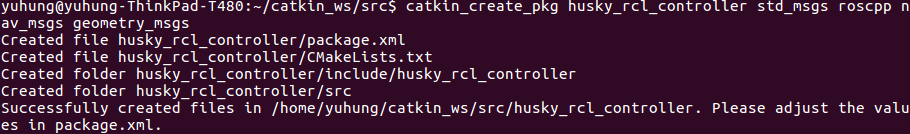
\includegraphics
            [width=1.0\textwidth]{./Figure/CreatePkg.png} %插入图片,[]中设置图片大小,{}中是图片文件名
            \vspace{-10mm}
            \caption{创建名为husky_rcl_controller的包} %最终文档中希望显示的图片标题
            \label{CreatePkg}
        \end{figure}
        \vspace{-4mm}
        重新编译工作空间,
        \vspace{-4mm}
        \begin{shaded}
            \noindent\verb|$ catkin build husky_rcl_controller|
        \end{shaded}
        \vspace{-4mm}
        更新环境变量,
        \vspace{-4mm}
        \begin{shaded}
            \noindent\verb|$ source ~/catkin_ws/devel/setup.bash|
        \end{shaded}
        \vspace{-4mm}
        搜索包并查找直接依赖项和全部依赖项({\ref{Rospack}}),
        \vspace{-4mm}
        \begin{shaded}
            \noindent\verb|$ rospack find husky_rcl_controller|\\
            \noindent\verb|$ rospack depends1 husky_rcl_controller|\\
            \noindent\verb|$ rospack depends husky_rcl_controller|
        \end{shaded}
        \vspace{-4mm}
        \begin{figure}[H]
			\centering
            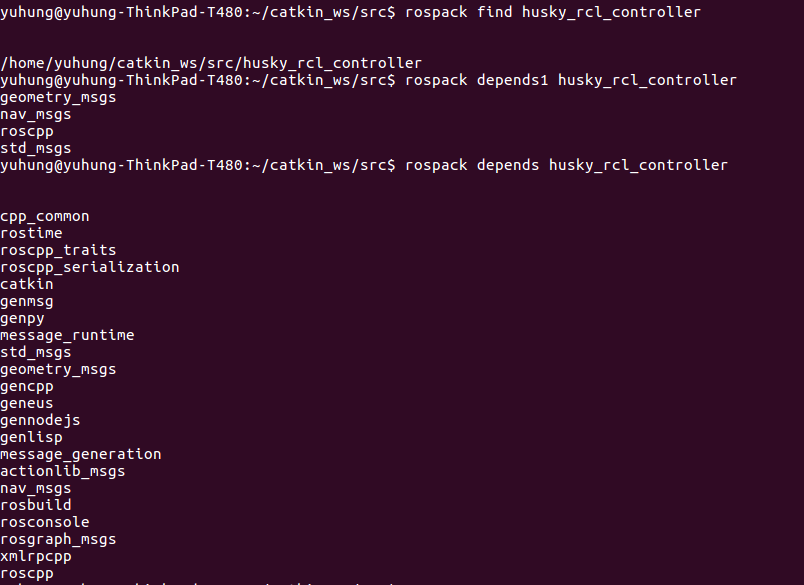
\includegraphics
            [width=1.0\textwidth]{./Figure/Rospack.png} %插入图片,[]中设置图片大小,{}中是图片文件名
            \vspace{-10mm}
            \caption{执行rospack相关命令} %最终文档中希望显示的图片标题
            \label{Rospack}
        \end{figure}
        \vspace{-4mm}
        \subsection{面向对象的ROS编程}
        \noindent
        1.查看/odometry/filtered消息的接收格式:

        先执行husky_empty_world仿真环境,
        \vspace{-4mm}
        \begin{shaded}
            \noindent\verb|$ roslaunch husky_gazebo husky_empty_world.launch|
        \end{shaded}
        \vspace{-4mm}
        利用rostopic命令行工具查看消息类型,
        \vspace{-4mm}
        \begin{shaded}
            \noindent\verb|$ rostopic type /odometry/filtered|
        \end{shaded}
        \vspace{-4mm}
        可以看到/odometry/filtered的消息类型是nav_msgs/Odometry({\ref{RostopicType}})。
        \vspace{-4mm}
        \begin{figure}[H]
			\centering
            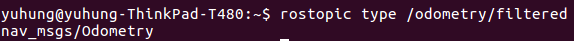
\includegraphics
            [width=1.0\textwidth]{./Figure/Rostopic.png} %插入图片,[]中设置图片大小,{}中是图片文件名
            \vspace{-10mm}
            \caption{执行rostopic查看消息类型} %最终文档中希望显示的图片标题
            \label{RostopicType}
        \end{figure}
        \vspace{-4mm}
        \noindent
        2.仿照teleop_twist_keyboard发布消息的模式,在算法类编写小车的控制算法,并在ROS类将控制的输出发送到话题:/cmd_vel:
        
        这里我们创建了算法类和Ros类,其各自的结构图({\ref{DataStruct}})如下:
        \vspace{-4mm}
        \begin{figure}[H]
            \centering
            \subfigure[]{
                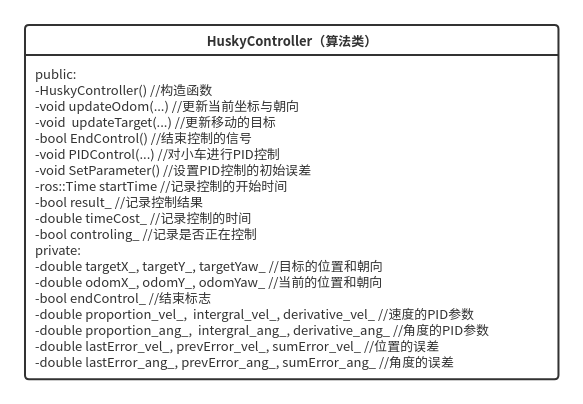
\includegraphics
                [width=0.4\textwidth]{./Figure/HuskyController.png}
            }
            \subfigure[]{
                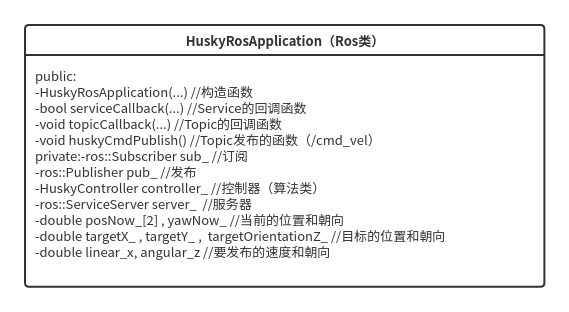
\includegraphics
                [width=0.5\textwidth]{./Figure/HuskyRosApplication.png}
            }
            \vspace{-4mm}
            \caption{算法类(a)和Ros类(b)的类结构图} %最终文档中希望显示的图片标题
            \label{DataStruct}
        \end{figure}
        \vspace{-4mm}
        控制器的部分采用PID控制,虽然只使用了PD的参数,但算法类中依然提供了PID的三个参数可以调整,具体的控制框图({\ref{ControllerStruct}})如下:
        \vspace{-4mm}
        \begin{figure}[H]
			\centering
            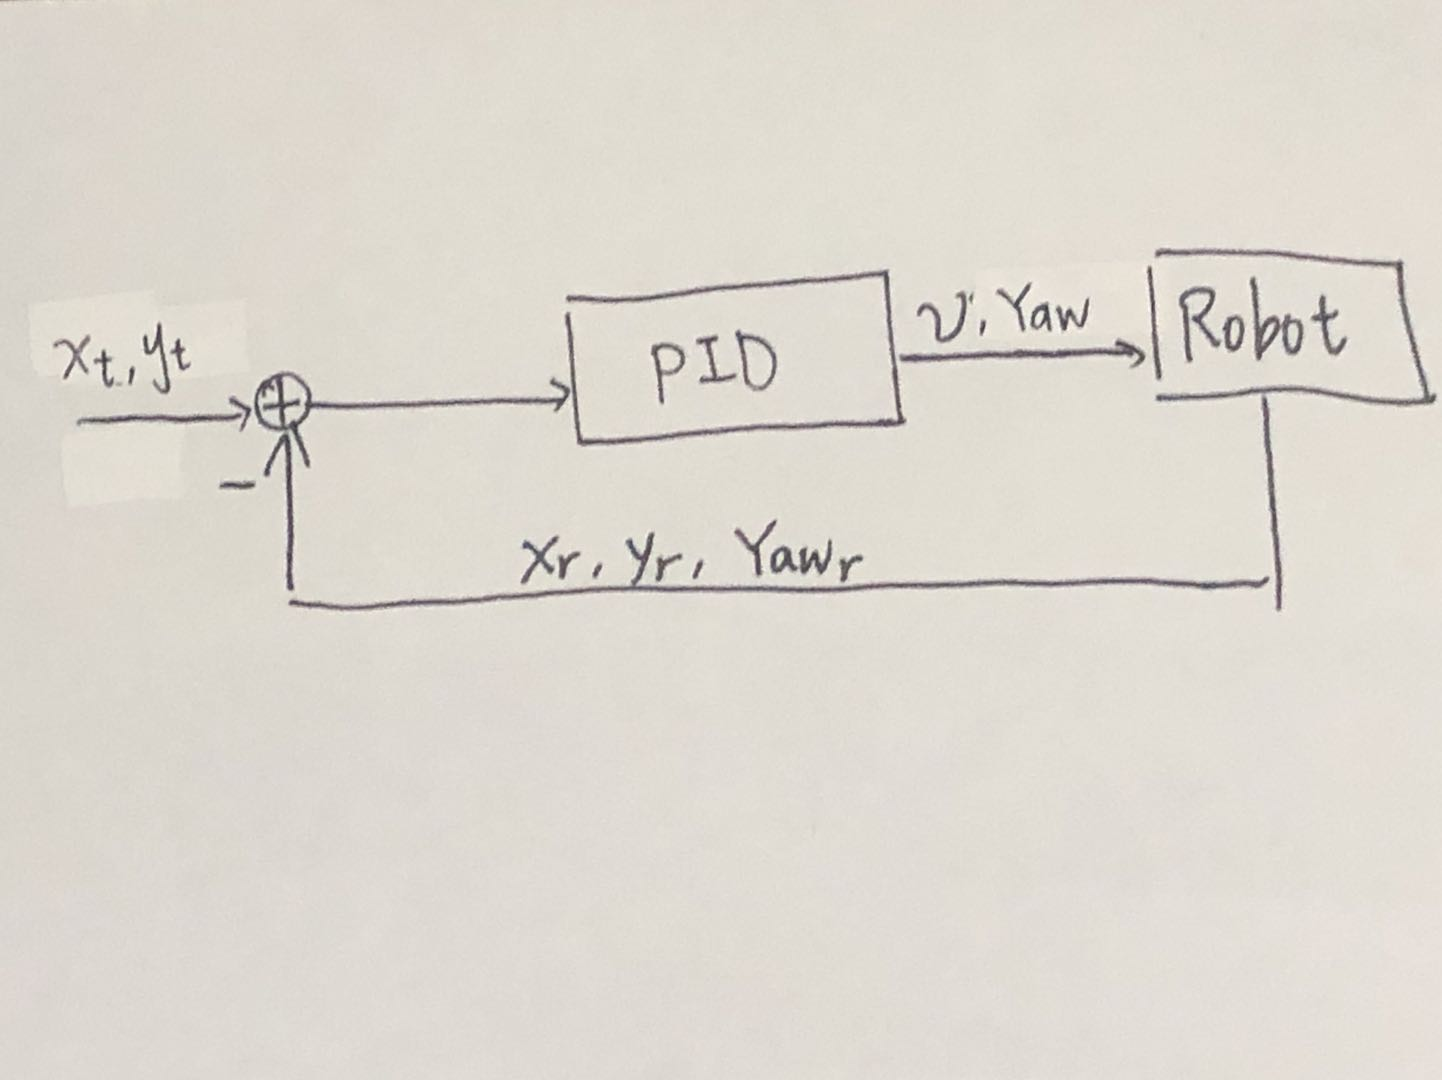
\includegraphics
            [width=0.6\textwidth]{./Figure/ControllerStruct.jpeg} %插入图片,[]中设置图片大小,{}中是图片文件名
            \vspace{-4mm}
            \caption{系统控制框图} %最终文档中希望显示的图片标题
            \label{ControllerStruct}
        \end{figure}
        \vspace{-4mm}
        其中$x_t,y_t$代表目标的位置(由于没有做挑战内容,所以没有目标的转向),$v,Yaw$代表发布的速度和角速度,$x_r,y_r,Yaw_r$代表实际机器人的位置和转向,透过反馈控制,控制机器人到达指定位置。

        检查rqt_graph(\ref{rqtGraph})可以看到,我们自己设计的控制器,的确满足要求向机器人发送/cmd_vel的消息并接收/odometry/filtered的消息。
        \vspace{-4mm}
        \begin{figure}[H]
			\centering
            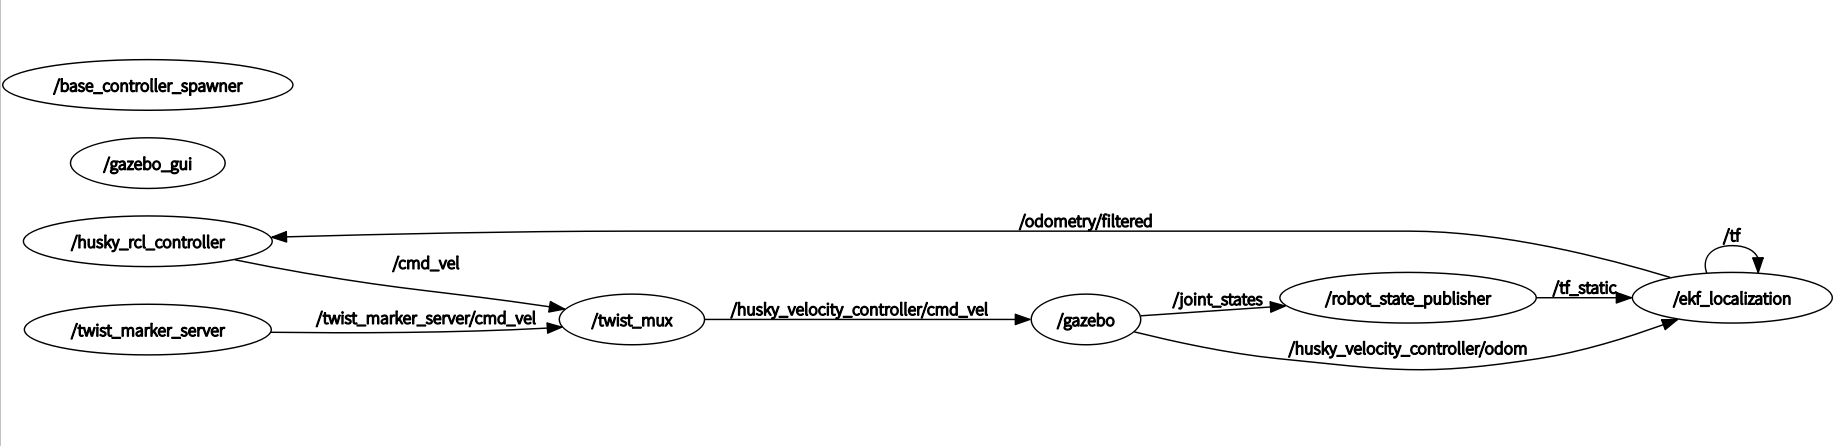
\includegraphics
            [width=0.8\textwidth]{./Figure/rqtGraph.png} %插入图片,[]中设置图片大小,{}中是图片文件名
            \vspace{-4mm}
            \caption{rqt_graph结果} %最终文档中希望显示的图片标题
            \label{rqtGraph}
        \end{figure}
        \vspace{-4mm}
        \noindent
        3.创建ROSServer:

        按照前一节的创建ROS package的方法,创建一个名为husky_rcl_controller_srv的包,在husky_rcl_controller_srv的目录下,创建srv文件夹,
        \vspace{-4mm}
        \begin{shaded}
            \noindent\verb|$ cd ~/catkin_ws/src/husky_rcl_controller_srv|\\
            \noindent\verb|$ mkdir srv|\\
            \noindent\verb|$ cd srv|
        \end{shaded}
        \vspace{-4mm}
        创建.srv文件,输入目标的消息格式({\ref{SrvType}}),
        \vspace{-4mm}
        \begin{shaded}
            \noindent\verb|$ vim husky_rcl_controller_srv.srv|
        \end{shaded}
        \vspace{-4mm}
        \begin{figure}[H]
			\centering
            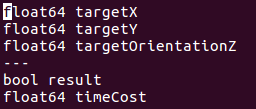
\includegraphics
            [width=0.5\textwidth]{./Figure/SrvType.png} %插入图片,[]中设置图片大小,{}中是图片文件名
            \vspace{-6mm}
            \caption{Srv文件中规定的图片格式} %最终文档中希望显示的图片标题
            \label{SrvType}
        \end{figure}
        \vspace{-4mm}
        分别修改package.xml({\ref{editPackage}})和CMakeLists.txt({\ref{editCMakeLists}})两个文件[1],
        \vspace{-4mm}
        \begin{shaded}
            \noindent\verb|$ cd ..|\\
            \noindent\verb|$ gedit package.xml|\\
            \noindent\verb|$ gedit CmakeLists.txt|
        \end{shaded}
        \vspace{-4mm}
        \begin{figure}[H]
			\centering
            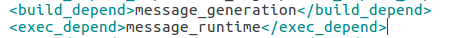
\includegraphics
            [width=1\textwidth]{./Figure/editPackage.png} %插入图片,[]中设置图片大小,{}中是图片文件名
            \vspace{-10mm}
            \caption{修改package.xml的内容,添加图中两行} %最终文档中希望显示的图片标题
            \label{editPackage}
        \end{figure}
        \vspace{-4mm}
        \begin{figure}[H]
            \centering
            \subfigure[]{
                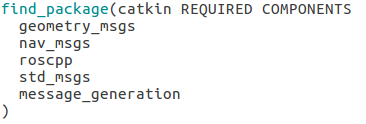
\includegraphics
                [width=0.5\textwidth]{./Figure/editCMakeLists1.png}
            }
            \subfigure[]{
                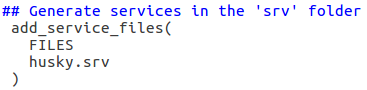
\includegraphics
                [width=0.5\textwidth]{./Figure/editCMakeLists2.png}
                \vspace{0mm}
                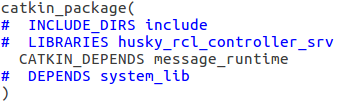
\includegraphics
                [width=0.5\textwidth]{./Figure/editCMakeLists3.png}
            }
            \vspace{-6mm}
            \caption{修改CMakeLists.txt的内容} %最终文档中希望显示的图片标题
            \label{editCMakeLists}
        \end{figure}
        \vspace{-4mm}
        更新环境变量,
        \vspace{-4mm}
        \begin{shaded}
            \noindent\verb|$ cd source ~/catkin_ws/devel/setup.bash|
        \end{shaded}
        \vspace{-4mm}
        检查server的消息格式({\ref{Rossrv}}),
        \vspace{-4mm}
        \begin{shaded}
            \noindent\verb|$ rossrv show husky_rcl_controller_srv|
        \end{shaded}
        \vspace{-4mm}
        \begin{figure}[H]
			\centering
            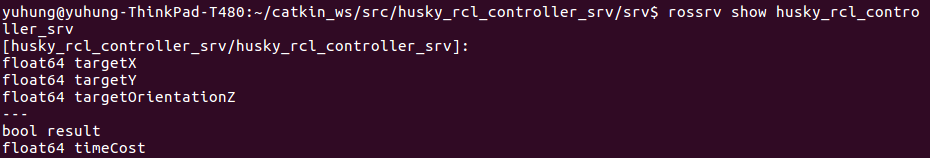
\includegraphics
            [width=1\textwidth]{./Figure/Rossrv.png} %插入图片,[]中设置图片大小,{}中是图片文件名
            \vspace{-10mm}
            \caption{检查server消息格式} %最终文档中希望显示的图片标题
            \label{Rossrv}
        \end{figure}
        \vspace{-4mm}
        \noindent
        4.使用命令行语句,手动输入参数,调用编写好的Service接口,完成让小车移动到指定位置的任务:

        首先我们要修改husky_rcl_controller下的CMakeLists.txt和package.html文件,找到对应内容并修改成以下形式,
        
        CMakeLists.txt:
\begin{lstlisting}[language=C]
cmake_minimum_required(VERSION 2.8.3)
project(husky_rcl_controller)
find_package(catkin REQUIRED COMPONENTS
    geometry_msgs
    nav_msgs
    roscpp
    std_msgs
    husky_rcl_controller_srv
)
catkin_package(
    INCLUDE_DIRS include
    CATKIN_DEPENDS geometry_msgs nav_msgs roscpp
     std_msgs husky_rcl_controller_srv
)
include_directories(
    include
    ${catkin_INCLUDE_DIRS}
)
add_executable(${PROJECT_NAME}
    src/HuskyRosApplication.cpp
    src/HuskyController.cpp
    src/main.cpp
)
target_link_libraries(husky_rcl_controller
    ${catkin_LIBRARIES}
)
\end{lstlisting}

        package.xml添加以下几行:
        \vspace{-4mm}
        \begin{shaded}
            \noindent\verb|<build_depend>husky_rcl_controller_srv</build_depend>|\\
            \noindent\small\verb|<build_export_depend>husky_rcl_controller_srv</build_export_depend>|\\
            \noindent\verb|<exec_depend>husky_rcl_controller_srv</exec_depend>|
        \end{shaded}
        \vspace{-4mm}
        对husky_rcl_controller包进行编译,
        \vspace{-4mm}
        \begin{shaded}
            \noindent\verb|$ catkin build husky_rcl_controller|
        \end{shaded}
        \vspace{-4mm}
        接下来开启仿真环境并运行自定义的Ros节点,
        \vspace{-4mm}
        \begin{shaded}
            \noindent\verb|$ roslaunch husky_gazebo husky_empty_world.launch|\\
            \noindent\verb|$ rosrun husky_rcl_controller husky_rcl_controller|
        \end{shaded}
        \vspace{-4mm}
        利用rosservice发布目标命令,并观察结果({\ref{RosService}}),
        \vspace{-4mm}
        \begin{shaded}
            \noindent\verb|$ rosservice call husky_rcl_controller/husky_controller_server|\\
            \noindent\verb|1 1 0|
        \end{shaded}
        \vspace{-4mm}
        \begin{figure}[H]
			\centering
            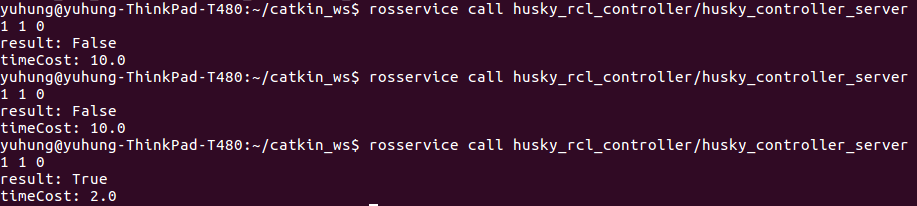
\includegraphics
            [width=1\textwidth]{./Figure/RosService.png} %插入图片,[]中设置图片大小,{}中是图片文件名
            \vspace{0mm}
            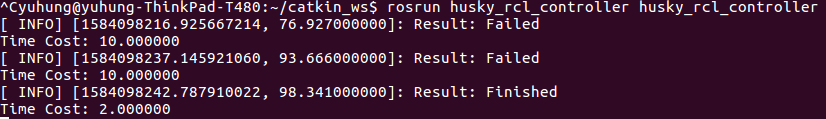
\includegraphics
            [width=1\textwidth]{./Figure/ROSINFO.png}
            \vspace{-10mm}
            \caption{执行三次目标命令分别的结果} %最终文档中希望显示的图片标题
            \label{RosService}
        \end{figure}
        \vspace{-4mm}
        利用rqt_plot显示控制结果({\ref{rqtPlot}}),
        \vspace{-4mm}
        \begin{shaded}
            \noindent\verb|$ rqt_plot|
        \end{shaded}
        \vspace{-4mm}
        \begin{figure}[H]
			\centering
            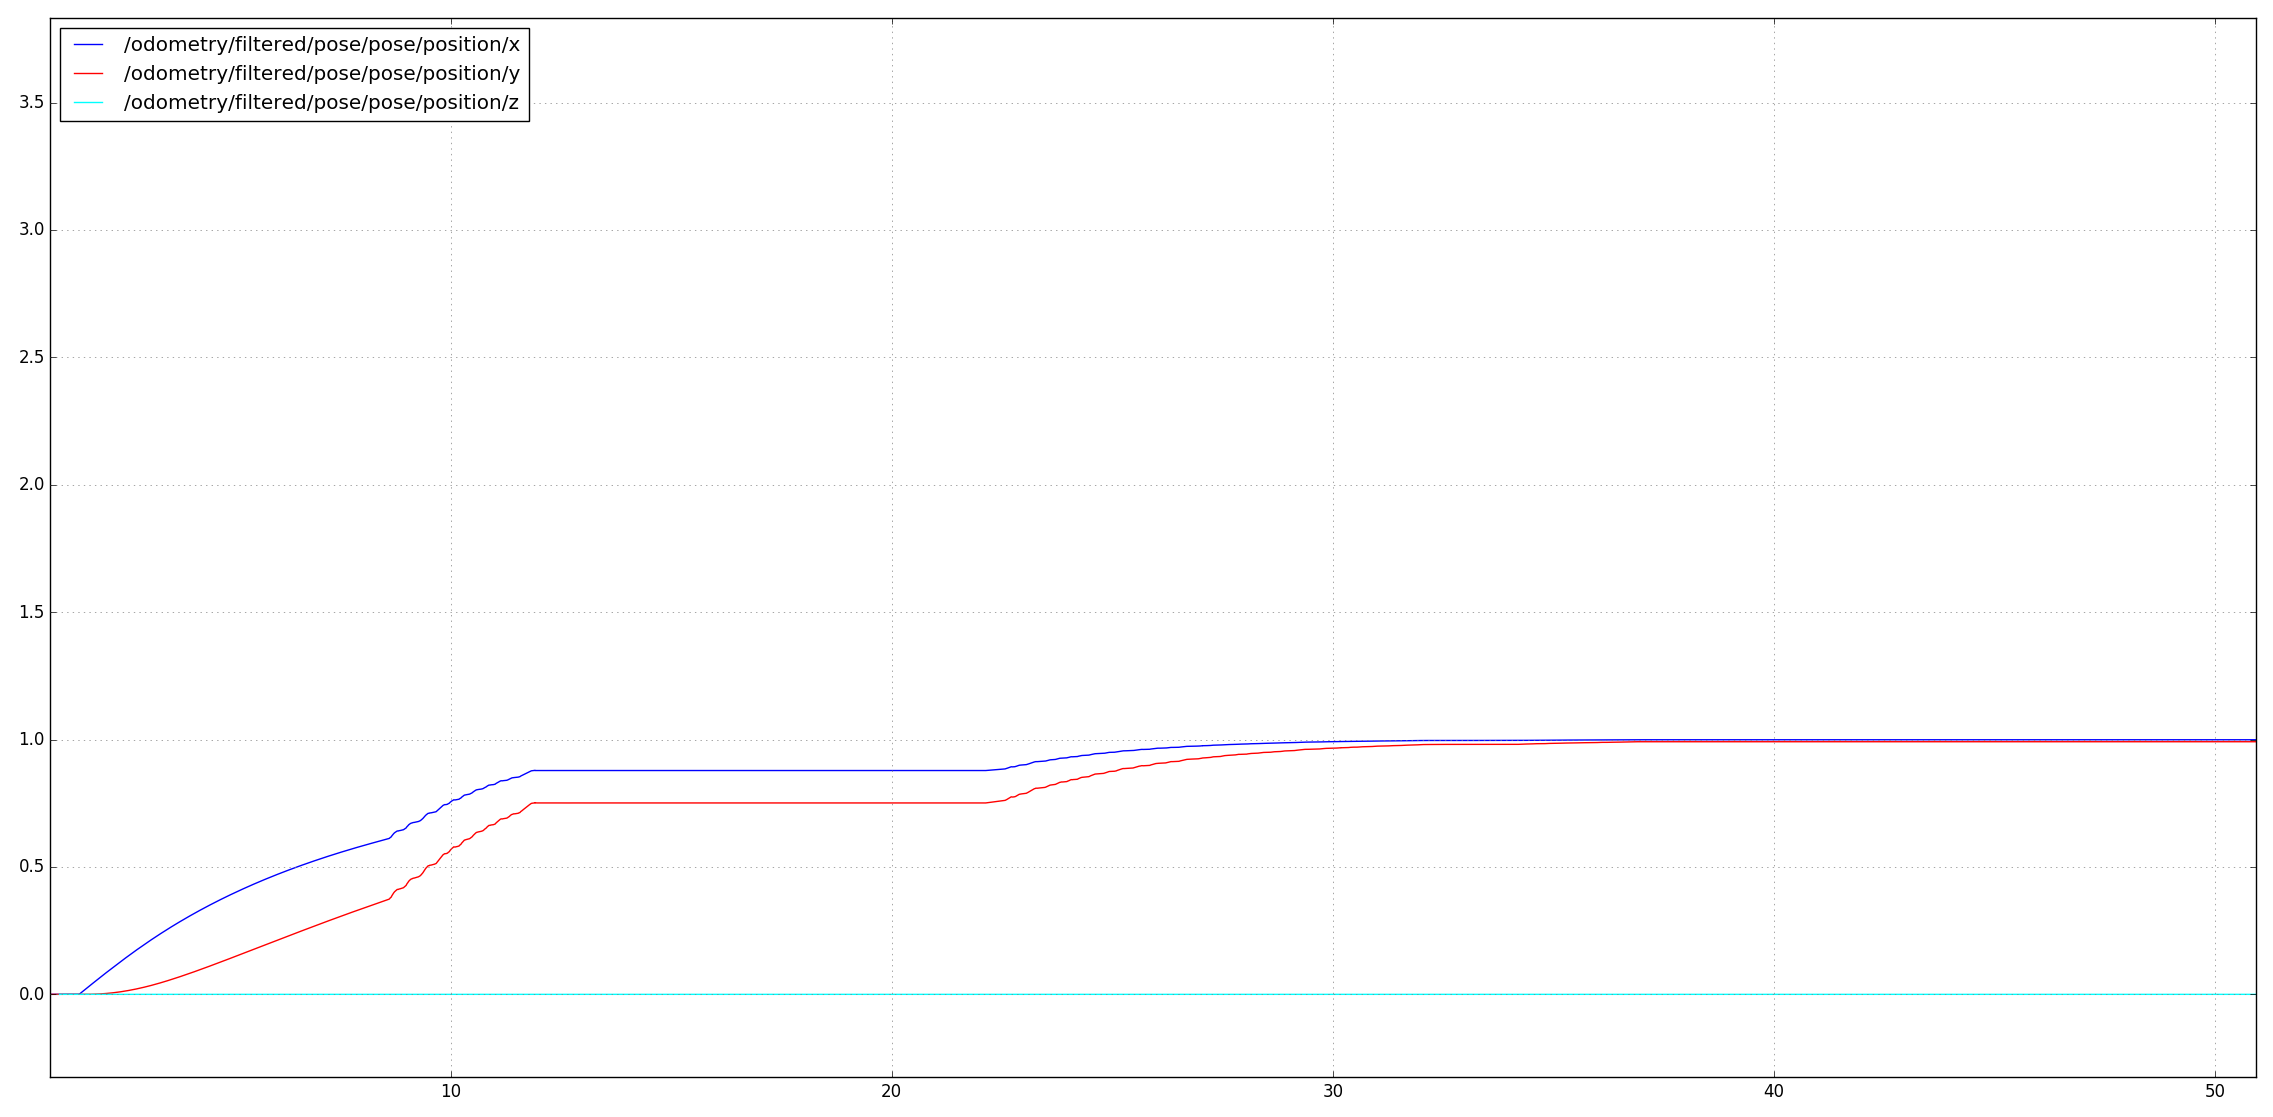
\includegraphics
            [width=1\textwidth]{./Figure/rqtPlot.png} %插入图片,[]中设置图片大小,{}中是图片文件名
            \vspace{-10mm}
            \caption{rqt_plot的控制效果曲线} %最终文档中希望显示的图片标题
            \label{rqtPlot}
        \end{figure}
        \vspace{-4mm}
    \vspace{-6mm}
		\subsection{对于Ros消息机制的理解}
            在Ros中,提供了两种不同的消息机制,分别是Topic和Service,Topic是透过发布者(Publisher)和订阅者(Subscriber)来进行通信,任何节点都可以是一个Topic的发送者或订阅者所以Topic的消息机制是一个多对多的机制,在Publisher中,只要根据指定Topic的数据格式定义要发送的数据,就可以发送一个Topic。而Subscriber是透过回调函数(Callback)接收想要订阅的Topic,将得到的数据再进行处理。
            
            Service机制则是一个一对一的消息机制,可以由用户定义发布的消息类型和回复的消息类型,利用客户端(Client)接收消息传送给服务端(Server),并由服务端经过自己内部的运算(回调函数Callback),返回结果给客户端。

            在本次的实验中,我们综合利用了两种消息机制,透过Service接收控制台的目标命令,在利用Topic机制来接收当前位置和控制结果(速度和角速度)。
    \vspace{-4mm}
    \section{参考文献}
    \noindent[1]\url{https://blog.csdn.net/u010647296/article/details/83143946?depth_1-utm_source=distribute.pc_relevant.none-task&utm_source=distribute.pc_relevant.none-task}\\
    \noindent[2]\url{https://www.jianshu.com/p/ed1d9a490bd1}\\
    \noindent[3]\url{https://github.com/leggedrobotics/ros_best_practices}\\
    \noindent[4]\url{https://blog.csdn.net/lin5103151/article/details/89893380}\\
\end{document}
